%!TEX root = ../MC_SS17.tex
\section{Einführung}
\label{sec:para1}
\nextlecture
\subsection*{Transformationelle Programme vs. reaktive Systeme}
\subsubsection*{Transformationelle Programme}
\begin{itemize}
	\item Aus einer Eingabe wird eine Ausgabe berechnet:
	\item[] 
	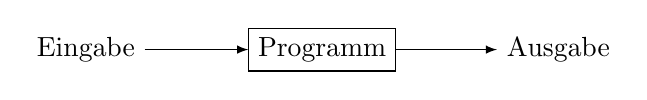
\begin{tikzpicture}
		\node[](eingabe) at (0,0) {Eingabe};
		\node[draw](programm) at (3,0) {Programm};
		\node[](ausgabe) at (6,0) {Ausgabe};
		
		\draw[-latex] (eingabe) to (programm);
		\draw[-latex] (programm) to (ausgabe);
	\end{tikzpicture}
	\item wird beispielsweise in der Algorithmik studiert
	\item typische Anforderung: Das Programm soll terminieren
	\item Klassische Programmverifikationsmethoden wie die Hoare-Logig oder die Methode von Floyd werden in den Vorlesungen \enquote{Theorie der Programmierung} und \enquote{Formale Methoden der Software-Entwicklung} behandelt.
\end{itemize}

\subsection*{Reaktive Systeme}
\begin{itemize}
	\item[] 
	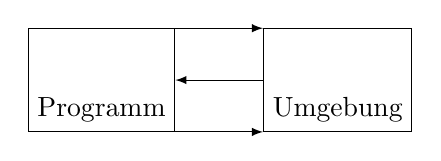
\begin{tikzpicture}
		\node[draw, text height = 1cm](programm) at (0,0) {Programm};
		\node[draw, text height = 1cm](umgebung) at (3,0) {Umgebung};
		
		\draw[-latex] (programm.north east) to (umgebung.north west);
		\draw[-latex] (umgebung.west) to (programm.east);
		\draw[-latex] (programm.south east) to (umgebung.south west);
	\end{tikzpicture}
	\item Programm steht in ständiger Interaktion mit seiner Umgebung
	\item Beispiele: Betriebssysteme, Netzwerkkontext, Kommunikationsprotokolle, Eingebettete Systeme: \underline{Ampel}, \underline{Flugzeug}, \underline{ABS}, Fernseher, Waschmaschine, \underline{Medizinische Geräte}, \dots
	\item[] \textunderscore: oft sicherheitskritisch $\Rightarrow$ Hohe Anforderung an Korrektheit
	\item Typisch für reaktive Systeme: Nicht terminierend
\end{itemize}

\subsection*{Model-Checking}
Die Idee von Model-Checking kann man im Allgemeinen an der folgenden Formel erkennen. Auf alle drei Teile der Formel wird im Laufe dieser Vorlesung eingegangen.
\begin{center}
	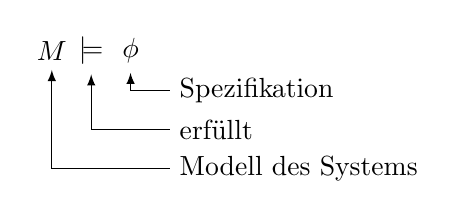
\begin{tikzpicture}
		\node[](m) at (0,0) {$M$};
		\node[](sat) at (0.5,0) {$\models$};
		\node[](phi) at (1,0) {$\phi$};
		
		\node[anchor = west](phi_hint) at (1.5,-0.5) {Spezifikation};
		\node[anchor = west](sat_hint) at (1.5, -1) {erfüllt};
		\node[anchor = west](m_hint) at (1.5, -1.5) {Modell des Systems};
		
		\draw[-latex] (phi_hint.west) -| (phi.south);
		\draw[-latex] (m_hint.west) -| (m.south);
		\draw[-latex] (sat_hint.west) -| (sat.south);
		\end{tikzpicture}
\end{center}	


\subsubsection*{Systemmodelle}
	Systeme werden automatenartig modelliert, meist mit endlichen vielen Zuständen. Beispiele:
	\begin{center}
		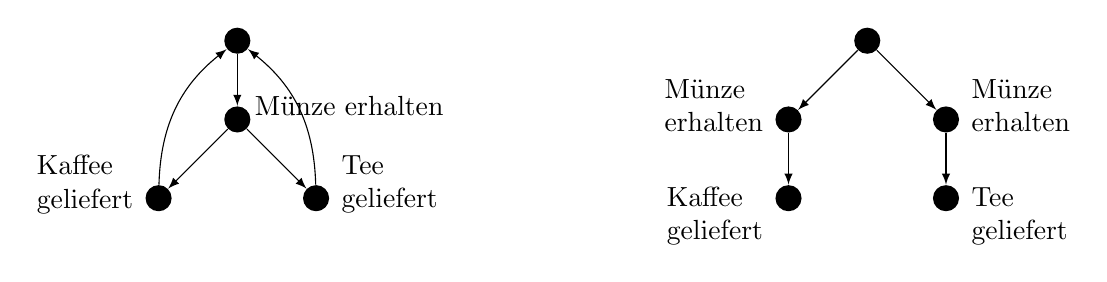
\begin{tikzpicture}
			\node[fill=black, circle](1_1) at (0,0) {};
			\node[fill=black, circle, label = {[align=left, right, xshift=1mm]Münze erhalten}](1_2) at (0,-1){};
			\node[fill=black, circle, label = {[align=left, xshift=-2mm,left]Kaffee\\geliefert}](1_3) at (-1,-2){};
			\node[fill=black, circle, label = {[align=left, xshift=2mm, right]Tee\\geliefert}](1_4) at (1,-2){};
			
			\draw[-latex] (1_1) to (1_2);
			\draw[-latex] (1_2) to (1_3);
			\draw[-latex] (1_2) to (1_4);
			\draw[-latex, bend left = 25] (1_3) to (1_1);
			\draw[-latex, bend right = 25] (1_4) to (1_1);
			
			
			
			\node[fill=black, circle](2_1) at (8,0) {};
			\node[fill=black, circle, label = {[align=left, xshift=-2mm, left]Münze\\erhalten}](2_2) at (7,-1) {};
			\node[fill=black, circle, label = {[align=left, xshift=-2mm,  yshift=-4mm,left]Kaffee\\geliefert}](2_3) at (7,-2) {};
			\node[fill=black, circle, label = {[align=left, xshift=2mm, right]Münze\\erhalten}](2_4) at (9,-1) {};
			\node[fill=black, circle, label = {[align=left, yshift=-4mm, xshift=2mm, right]Tee\\geliefert}](2_5) at (9,-2) {};
			\node[](2_sub) at (6,-1.5) {};
			
			\draw[-latex] (2_1) to (2_2);
			\draw[-latex] (2_1) to (2_4);
			\draw[-latex] (2_2) to (2_3);
			\draw[-latex] (2_4) to (2_5);
		\end{tikzpicture}
		\todo{Pfeile im zweiten Bild}
	\end{center}

\subsubsection*{Spezifiaktionen}
	Die Spezifikationen werden in Form von Temporal-logische Formeln angegeben. Beispiele:
	\begin{enumerate}[a)]
		\item $\phi_{\text{Tee}} =_{\text{def}} \text{EF}(\text{Tee geliefert})$ \hspace{2cm}\enquote{Der Automat kann Tee liefern}
		
		Beide Beispielmodelle erfüllen die Formel.
		
		\item $\phi_{\text{happy}} =_{\text{def}} \text{AG}(\text{Münze erhalten} \Rightarrow \text{EX Kaffee geliefert})$ \hspace{2cm}\enquote{Immer wenn der Automat eine Münze erhalten hat, kann er im nächsten Schritt Kaffee liefern.}
		
		Nur das erste Beispielmodell erfüllt diese Formel, das zweite nicht.
	\end{enumerate}

\subsection*{Methoden zur Validierung von Systemen/Programmen}
\subsubsection*{Testen}
\begin{itemize}
	\item[+] Relativ einfach durchzuführen
	\item[+] Oft sehr effektiv zum Fehlerfinden
	\item[-] Fundamental unvollständig; nur die getesteten Durchläufe werden überprüft
\end{itemize}

\subsubsection*{Simulation}
Testdurchläufe mit einem Modell des Systems
\begin{itemize}
	\item[+/-] wie beim Testen
	\item[+] Fehlerfinden bevor das System gebaut wird
\end{itemize}

\subsubsection*{Codereviews/Code-Inspektion}
Programm wird von unabhängigen (Team von) Code-Inspektoren überprüft
\begin{itemize}
	\item[+] oft sehr effektiv, Delegation von Verantwortung
	\item[-] teuer
	\item[-] i.A. unvollständig
\end{itemize}

\subsubsection*{Verifikation}
Nachweis der Gültigkeit von Spezifikation mit mathematischen/logischen Methoden
\begin{itemize}
	\item[+] Alle Ausführungspfade werden überprüft (Mögliches Problem: Differenzen zwischen verifizierten Modell und Implementierung)
\end{itemize}
Es gibt verschiedene Arten der Verifikation, die im folgenden diskutiert werden.

\begin{enumerate}[a)]
	\item \emph{Deduktive Verifikation:} Anwendung von Beweiskalkülen (Axiome und Schlussregeln)
	\begin{itemize}
		\item[+] komplexe Spezifikationen können nachgewiesen werden
		\item[-] aufwending
		\begin{itemize}
			\item[] nur teilweise automatisierbar
			\item[] $\rightarrow$ schwer wiederholbar
			\item[] $\rightarrow$ kann zu Erstarrung des Systemdesigns führen
			\item[] Aber: großer Fortschritt bei Theorembeweisen relativiert die Nachteile zum Teil
		\end{itemize}
	\item[-] bei rein manueller Durchführung: Korrektheit der Beweisführung problematisch
	\end{itemize}

	\item \emph{Automatische Verifikation:} Anwendung algorithmischer Verifikationsverfahren
	\begin{itemize}
		\item[+] im Prinzip vollautomatisch (\enquote{Push-Button-Verifikation}) $\rightarrow$ billig, leicht wiederholbar
		\item[-] schwächere Spezifikation als bei deduktiver Verifikation
		\item[-] \savepos{a} Korrektheit des Verifikationswerkzeug kann problematisch sein, es gibt aber Gegenmaßnahmen
		\hfill\savepos{b}
		    \begin{tikzpicture}[remember picture, overlay]
		\path (a) ++(-\labelwidth,\ht\strutbox) coordinate (x) ;
		\path (b) ++(1em,-\dp\strutbox) coordinate (y) ;
		\draw (x |- y) to[out=100,in=260] (x) ;
		\draw (x -| y) to[out=280,in=80] (y) ;
		\end{tikzpicture}
		
	\end{itemize}
\end{enumerate}

\subsection*{Theorem von Rice}
\underline{Alle} nicht-trivialen Eigenschaften von Programmen universeller Programmiersprachen sind unentscheidbar.

Konsequenz: \underline{Volle automatische} Verifikation für \underline{berechnungsuniverselle} Programmiersprache ist unmöglich. Daraus ergeben sich zwei mögliche Auswege:

\begin{enumerate}
	\item Verifikationsalgorithmus ist partiell: sagt manchmal \enquote{weiß ich nicht} oder der Algorithmus terminiert nicht. Beispiel: Analyse in Codeoptimierern. Mehr in der Vorlesung \enquote{Theorie der Programmierung}
	\item Verifikationsalgorithmus wird auf nicht berechnungsuniversellen Formalismus angewandt: z.B. \enquote{Model Checking }
\end{enumerate}
\cleardoubleoddemptypage